% !TEX program = xelatex

\documentclass[a4paper,14pt,oneside,final]{extarticle}
% \usepackage[top=2cm, bottom=2cm, left=3cm, right=1cm]{geometry}
\usepackage{scrextend}

% Header and footer:
% display page number on top|right of the page
\usepackage{fancyhdr}
\pagestyle{fancy}
\fancyhf{}
\rhead{\small \selectfont \thepage}
\renewcommand{\headrulewidth}{0pt}

\usepackage{float}
\usepackage{pgfplots}
\usepackage{graphicx}
\usepackage{multirow}
\usepackage{amssymb,amsfonts,amsmath,amsthm}
\usepackage{csquotes}

\usepackage{listings}
\lstset{basicstyle=\footnotesize\ttfamily,breaklines=true}
\lstset{language=Matlab}

\usepackage[
	backend=biber,
	sorting=none,
	language=auto,
	autolang=other
]{biblatex}
\DeclareFieldFormat{labelnumberwidth}{#1}


\usepackage{systeme}
\usepackage{longtable,tabu}
\usepackage{multirow}
\usepackage{array,multirow}
\usepackage{pdflscape}
\usepackage{afterpage}
\usepackage{bm}
\usepackage{titling}
\usepackage{framed}

\graphicspath{{figures/}}
\addbibresource{bibliography.bib}

\title{Developing Adaptive Learning Management Application for Building Effective Project Team in IT-Industry}
\author{V. Karnaukh, M. Tkachuk, V. Sokol, M. Bilova}

\begin{document}

\maketitle

\begin{abstract}
IT-sphere is one of the most dynamic industries in the 21st century.  Therefore, to be successful, IT-companies should move with the times and keep their employees tuned. In order to reach this goal, an existing e-learning software was upgraded by developing a program module that enables project management to improve the efficiency of the project team’s selection in IT-industry. 

This work addresses the following tasks: identifying key Learning Management Systems that are used for corporate training, analyzing and comparing them, identifying the main weaknesses of existing systems and developing software for improving such systems. 

As a result, Open Olat LMS was chosen for the experiment dedicated to the integration of the developed program module for adaptive learning. This investigation has shown significant improvement in user experience and resource management processes. 
\end{abstract}

\section{Introduction}
The learning  management system concept emerged directly from e-Learning. Although the first LMS appeared in the higher education sector, the majority of the LMSs today focus on the corporate market. 

However, Learning Management Systems have not yet reached the eLearning marketplace to provide lifelong professional development, especially for the specific IT-market that demands from developers a broad and extendable skill set. IT companies are forced to create their own LMS for managing talents and assigning appropriate employees on the upcoming projects. This approach is time-consuming and requires additional resources for the development and support effort. 

Considering this fact, it’s crucial to improve the existing software by automating and accelerating employee training for IT based on specific project requirements. Talent management systems can be useful for accomplishing this task, helping recruiters and training professionals to develop and retain people with the necessary abilities or skills. 

Combining these systems by making learning content adaptive and based on individual needs enables resource managers to shorten the time needed for preparing specialists, improve staff skills effectively and reduce the cost of training. 

The key question to be answered in this paper is how to construct adaptive learning module and inject it into the existing architecture and which communication channels between systems should be used in order to be consolidated into a coherent whole.

\section{Literature review}
Unlike the regular education system, the goal of corporate training is related, first and foremost, to return on investment, namely using the knowledge acquired in the process of learning~\cite{Bakar2017KnowledgeRI}. An employee at an IT company acts as the principal asset for the technological features of curriculum design and development not only to ensure effective training, the stability of the acquired knowledge and skills, as well as the opportunity to participate in more complex and cost-effective projects. 

E-learning can be defined as any development practice that is delivered via the Internet or other e-learning source of information~\cite{HaveYouGot}. It is an online learning system that involves the use of a computer, laptop, or any electronic device and can continuously acquire knowledge and skills through learning events that are formed, delivered, supported by web technologies. E-training is considered as part of e-learning, which is more practical in nature and involves the use of acquired knowledge in specific examples~\cite{Pedro}.

The benefits of e-learning and e-training include the following.
\begin{enumerate}
    \item Ability to study anytime, anywhere~\cite{Successful,Implementing,Batalla-Busquets2013}.
    \item The sequence of training~\cite{Implementing}.
    \item Availability of access to a comprehensive archive of course content and its timely updates on a continuous basis~\cite{Successful,Batalla-Busquets2013}.
    \item Save time and minimize job separation~\cite{Burgess2003}.
    \item Economy by reducing the cost of travel for employees~\cite{Successful,Implementing}.
    \item Increasing productivity, improving training activities, return on investment~\cite{Successful,Burgess2003}.
    \item Increasing the level of satisfaction of employees and customers~\cite{Implementing,Gwebu2007}.
    \item Improvement of skills and knowledge of employees~\cite{Successful,Implementing}.
\end{enumerate}

At the same time, they point out the disadvantages of using e-learning, which include technical issues related to technology compatibility, poor internet connection, etc .; high cost of development and support; organizational problems~\cite{Implementing}.

Despite the drawbacks, eLearning has become an alternative form of acquisition of IT knowledge and practical skills through technological innovation and modern communication systems. Increasing use of this type of training has an impact on the work environment due to the system's compliance with scalability, access and timeliness requirements~\cite{Corporate}.

Typical LMS functionality provides the following: user registration; maintaining a course catalog; maintaining and providing access to the content and materials of e-learning and training courses; downloading e-learning modules and tools for staff; dissemination of educational material; management of educational materials; integration of knowledge management resources; checking and evaluating students; tracking and recording student outcomes and progress; tracking training activities; providing management training reports; the ability to chat, etc.~\cite{elearning,Encyclopedia,CMS}.

However, the main feature is absent in typical LMS – adaptive learning. Adaptive learning, also known as adaptive teaching, is an educational method which uses computer algorithms to orchestrate the interaction with the learner and deliver customized resources and learning activities to address the unique needs of each learner. In professional learning contexts, individuals may "test out" of some training to ensure they engage with novel instruction. Computers adapt the presentation of educational material according to students' learning needs, as indicated by their responses to questions, tasks and experiences. The next chapter describes main technologies and methodologies used for implementing adaptive learning for LMS. 

\section{Methods}
Adaptive learning systems have traditionally been divided into separate components or 'models'. While different model groups have been presented, most systems include some or all of the following models (occasionally with different names)~\cite{Facilitating,Noura}:
\begin{itemize}
    \item Expert model – The model with the information which is to be taught
    \item Student model – The model which tracks and learns about the student
    \item Instructional model – The model which actually conveys the information
    \item Instructional environment – The user interface for interacting with the system
\end{itemize}

In the developed application student model is used. The simplest means of determining a student's skill level is the method employed in CAT (computerized adaptive testing). In CAT, the subject is presented with questions that are selected based on their level of difficulty in relation to the presumed skill level of the subject. As the test proceeds, the computer adjusts the subject's score based on their answers, continuously fine-tuning the score by selecting questions from a narrower range of difficulty.

An algorithm for a CAT-style assessment is simple to implement. A large pool of questions is amassed and rated according to difficulty, through expert analysis, experimentation, or a combination of the two. The computer then performs what is essentially a binary search, always giving the subject a question which is halfway between what the computer has already determined to be the subject's maximum and minimum possible skill levels. These levels are then adjusted to the level of the difficulty of the question, reassigning the minimum if the subject answered correctly, and the maximum if the subject answered incorrectly.

CAT successively selects questions for the purpose of maximizing the precision of the exam based on what is known about the examinee from previous questions. This perfectly fits the issue to solve. 

Besides, due to certain shortcomings of existing LMSs and certain prospects for their improvement, the paper proposes to formulate an algorithm for testing an employee and for him to choose an adaptive program of training in applying graph theory.

Graph theory is a section of mathematics that studies the properties of graphs. Graphically, a graph can be imagined as a geometric configuration consisting of points (vertices) connected by lines (edges).

The structure of the organization of knowledge and competencies of the staff can be conveniently represented with the help of a directional tree.

Oriented (directed) tree is an acyclic digraph in which only one vertex has zero half-degree of input, and all other vertices have half-degree of input 1.

The root of the tree is a position that is likely to be given to an employee. The connecting vertices of the root are the so-called vertices of the first level, namely, the level of competence. The European Competence System was applied to select competences and relevant skills.

The European Competence System (e-CF) provides an accessible and detailed description of competences used in the IT field, using a common language for competences, skills, knowledge and levels of knowledge, providing a common understanding of them for European organizations.

The letters of the graph define the final knowledge that corresponds to certain skills. This is shown on the figure~\ref{fig:1}.

\begin{figure}[H]
    \centering
    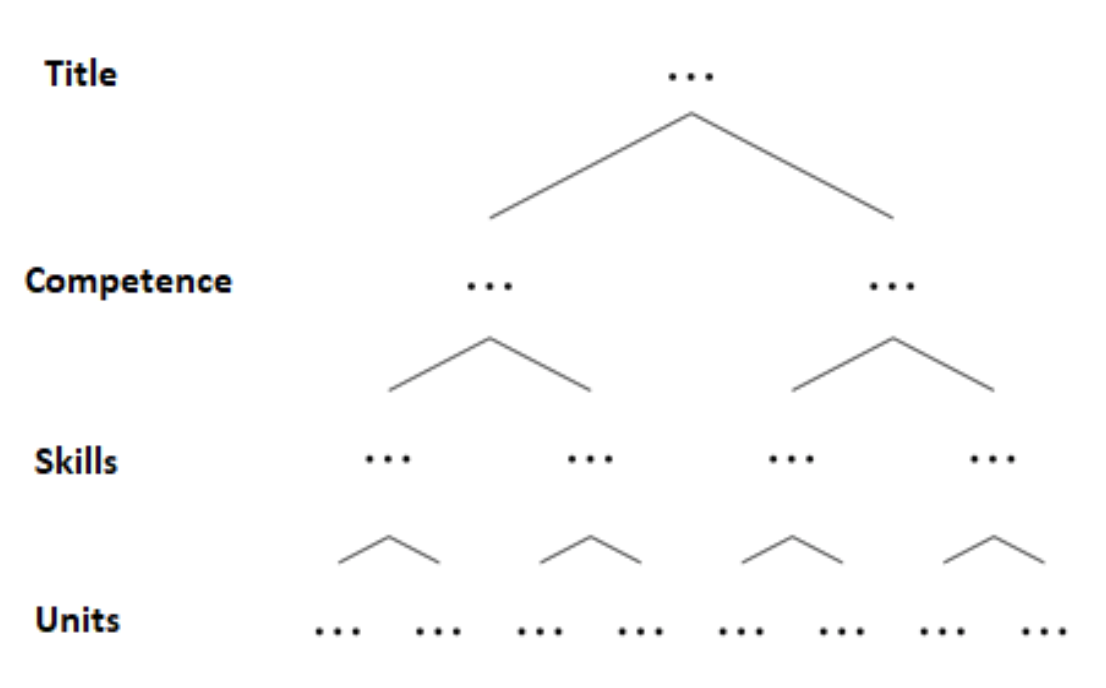
\includegraphics[width=0.75\textwidth]{fig1}
    \caption{Graph that represents relation of competence to skills}
    \label{fig:1}
\end{figure}

A label is added to the top of the graph model - the minimum knowledge threshold needed to create an individual refinement plan, as in figure~\ref{fig:2}.

\begin{figure}[H]
    \centering
    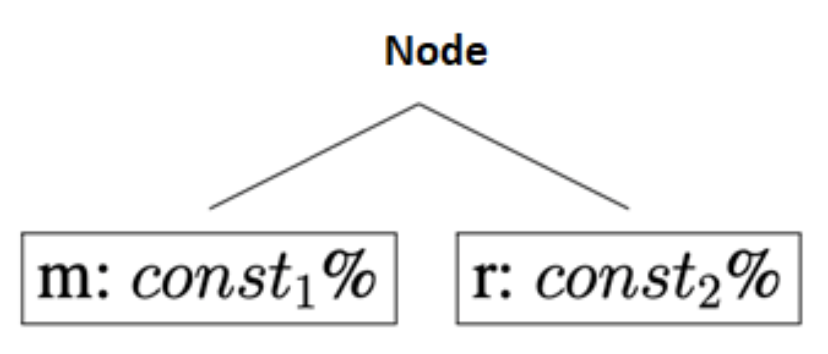
\includegraphics[width=0.5\textwidth]{fig2}
    \caption{Graph node structure}
    \label{fig:2}
\end{figure}

Property m means minimum knowledge threshold. Property r indicates the required level of knowledge to work on the project. The $const_1$ and $const_2$ variables are arbitrary numbers where $0\% \leq const_1 < const_2 \leq 100\%$.

The search algorithm can be represented by the following diagram in figure~\ref{fig:3}.

\begin{figure}[H]
    \centering
    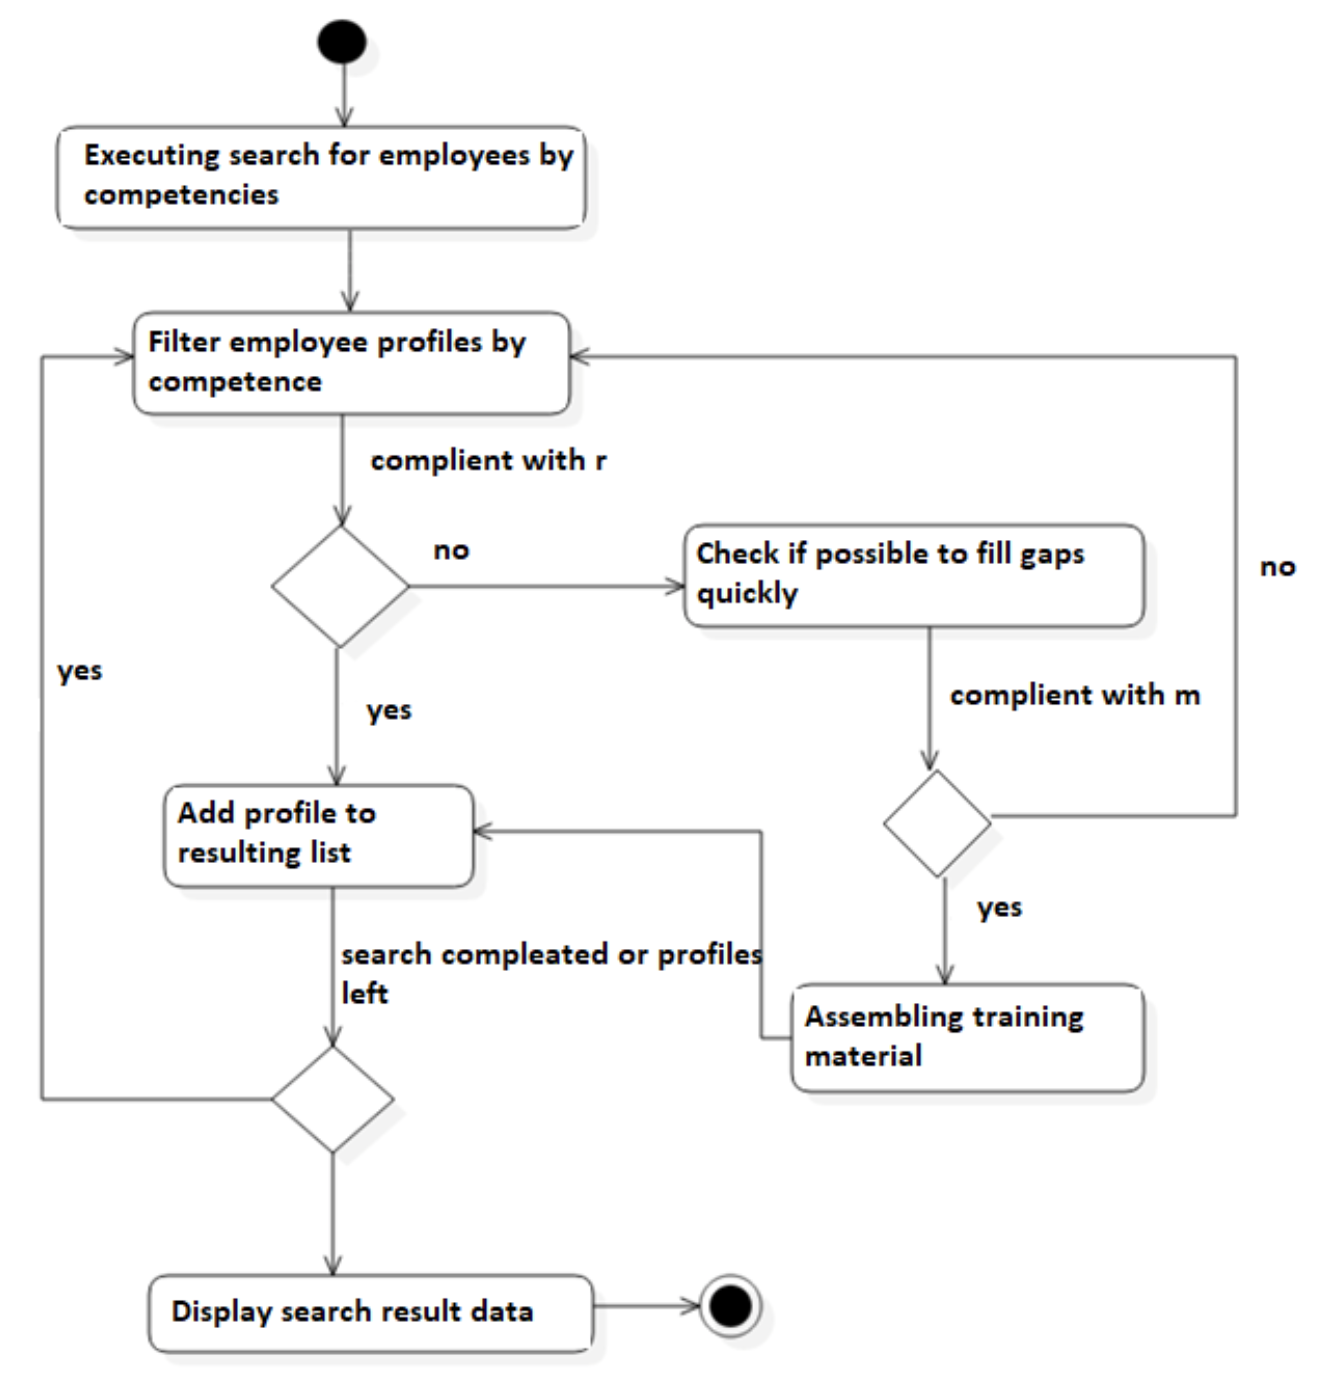
\includegraphics[width=0.6\textwidth]{fig3}
    \caption{Searching algorithm for employees by competence}
    \label{fig:3}
\end{figure}

To describe the business processes of the software, an information model was created in IDEF0, which is shown in the figure~\ref{fig:4}.

\begin{figure}[H]
    \centering
    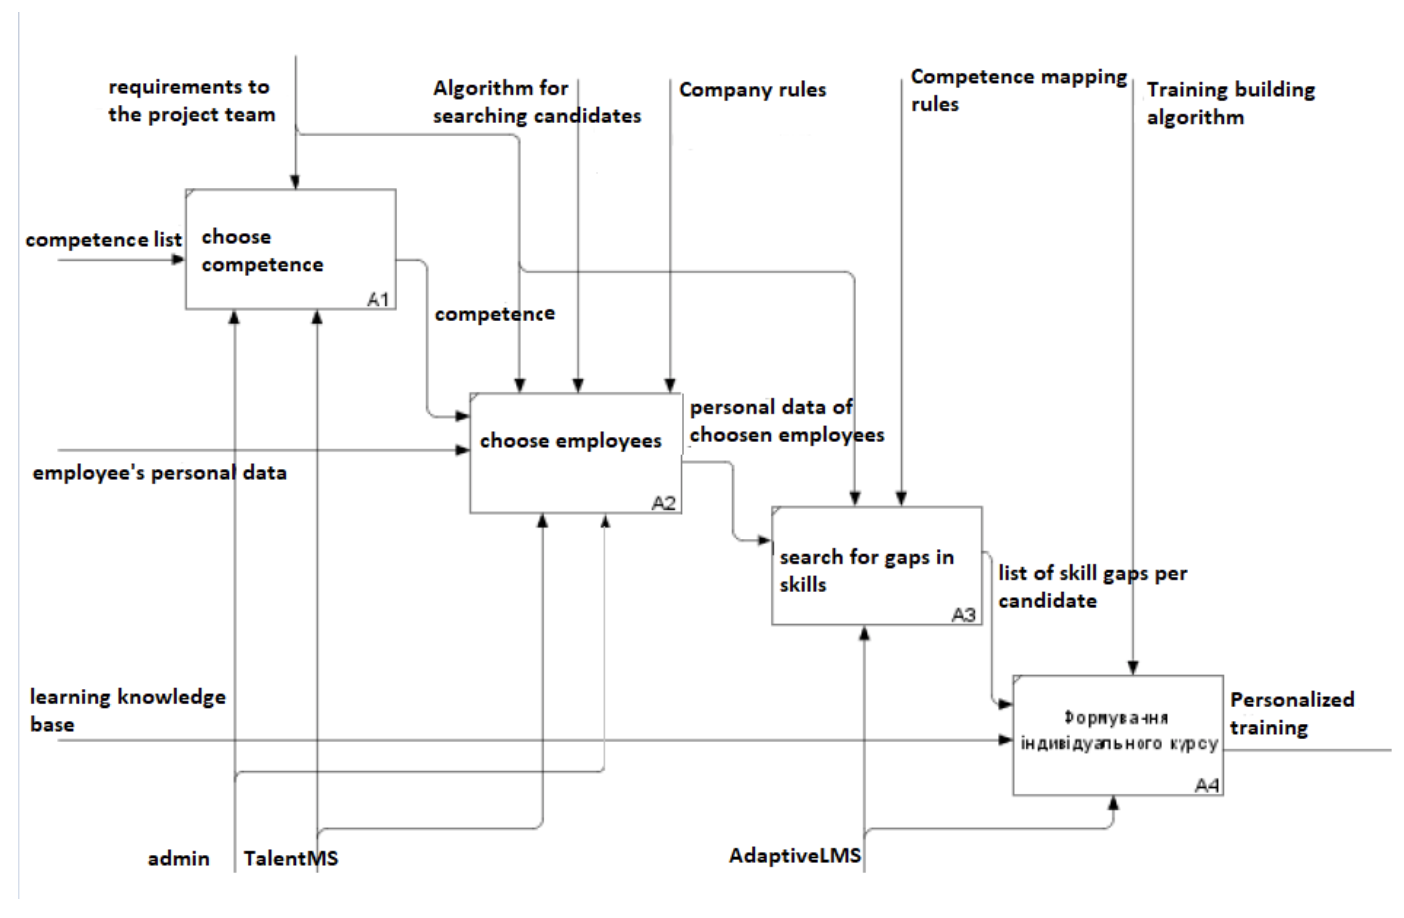
\includegraphics[width=1\textwidth]{fig4}
    \caption{Decomposed IDEF0 diagram for building personalized training process}
    \label{fig:4}
\end{figure}

\section{Results}
As a result, the application for talent management in IT companies was developed, including learning management, adaptive content and testing content modules. 

Main components of the application are shown on the diagram represented by figure~\ref{fig:5}.

\begin{figure}[H]
    \centering
    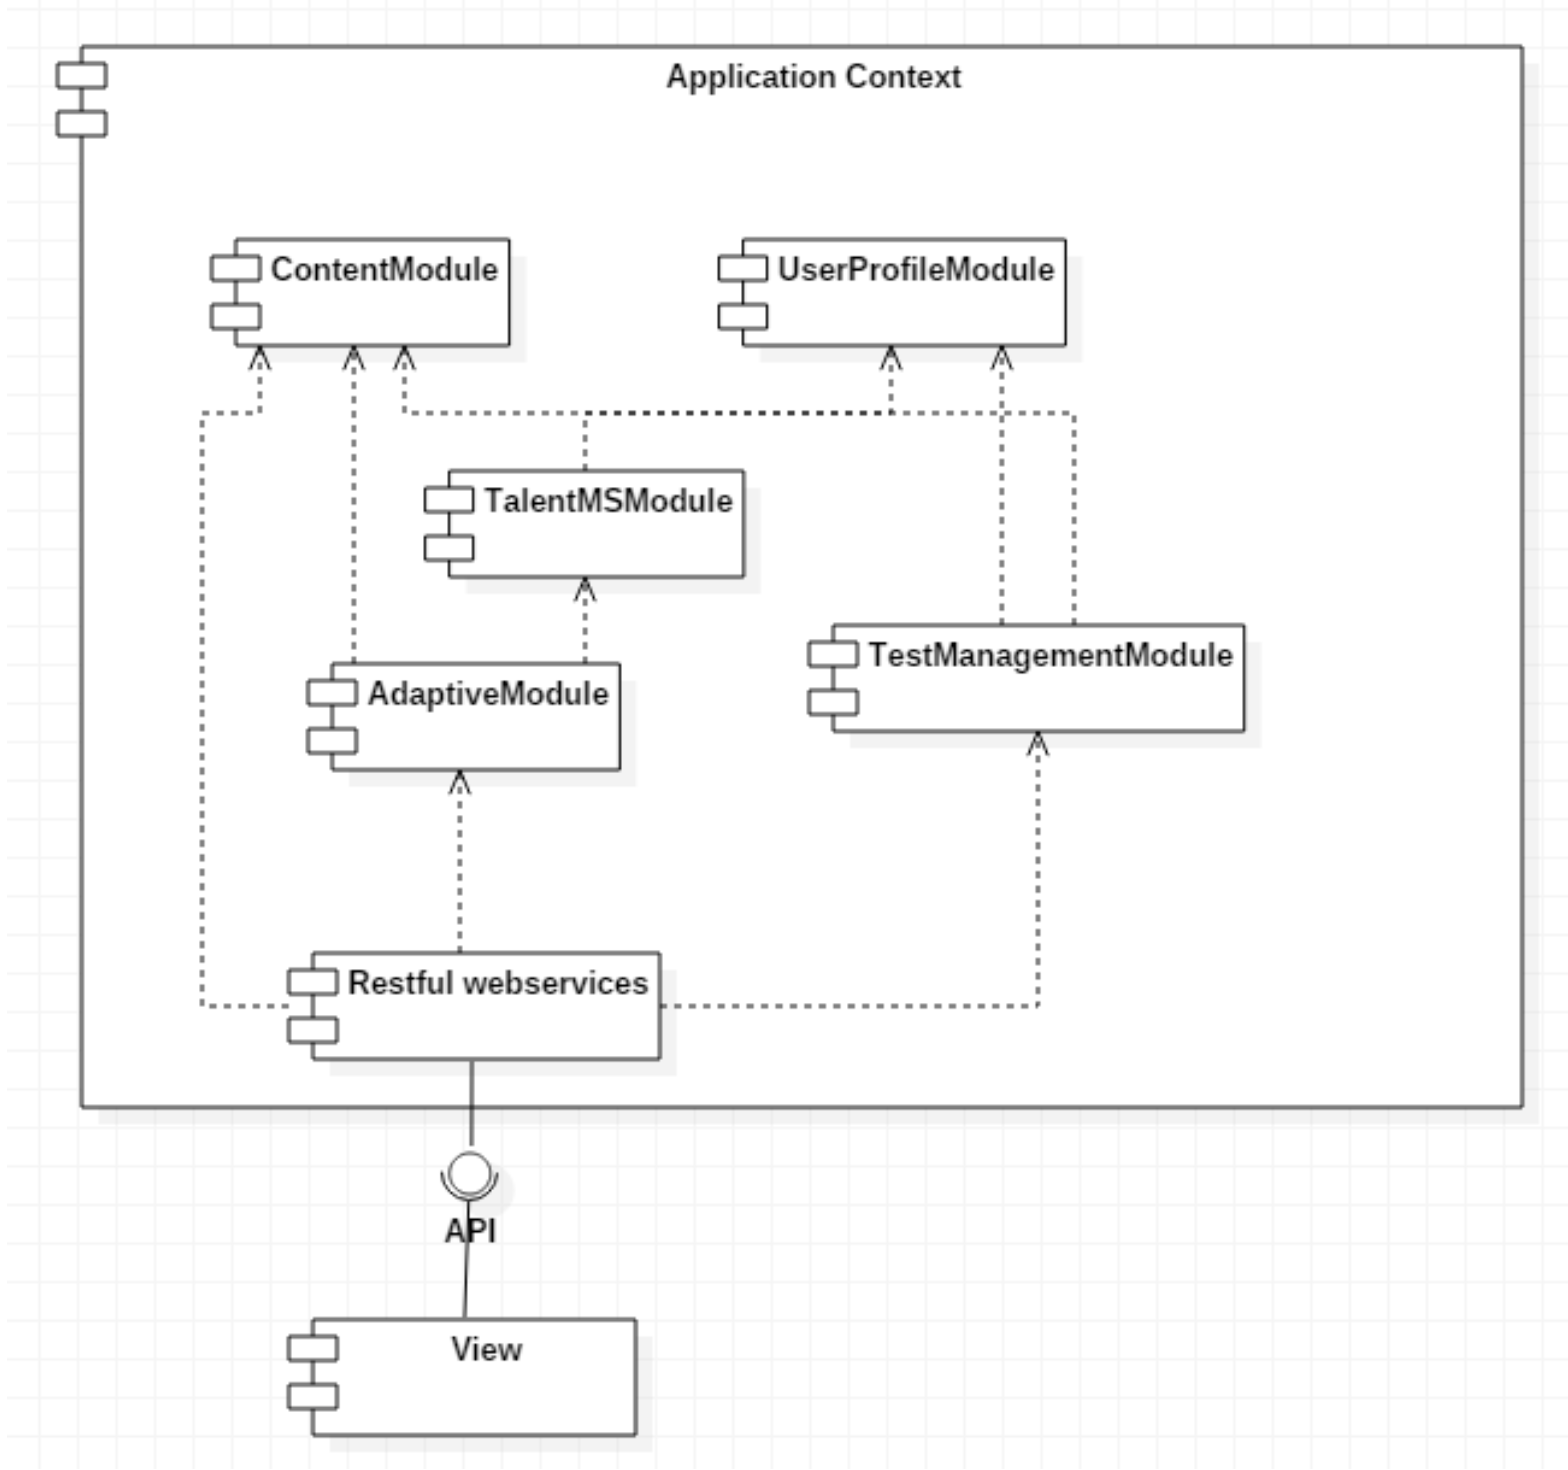
\includegraphics[width=1\textwidth]{fig5}
    \caption{Application component diagram}
    \label{fig:5}
\end{figure}

As can be observed from the diagram, there are also modules for content and user profile management, they are taken as is from OpenOLAT LMS. The communication with modules between channels is implemented with RESTful API approach that is used by view component. 

On the following diagram, that is represented on the figure~\ref{fig:6}, there is a sequence diagram dedicated to the test set building process. 

\begin{figure}[H]
    \centering
    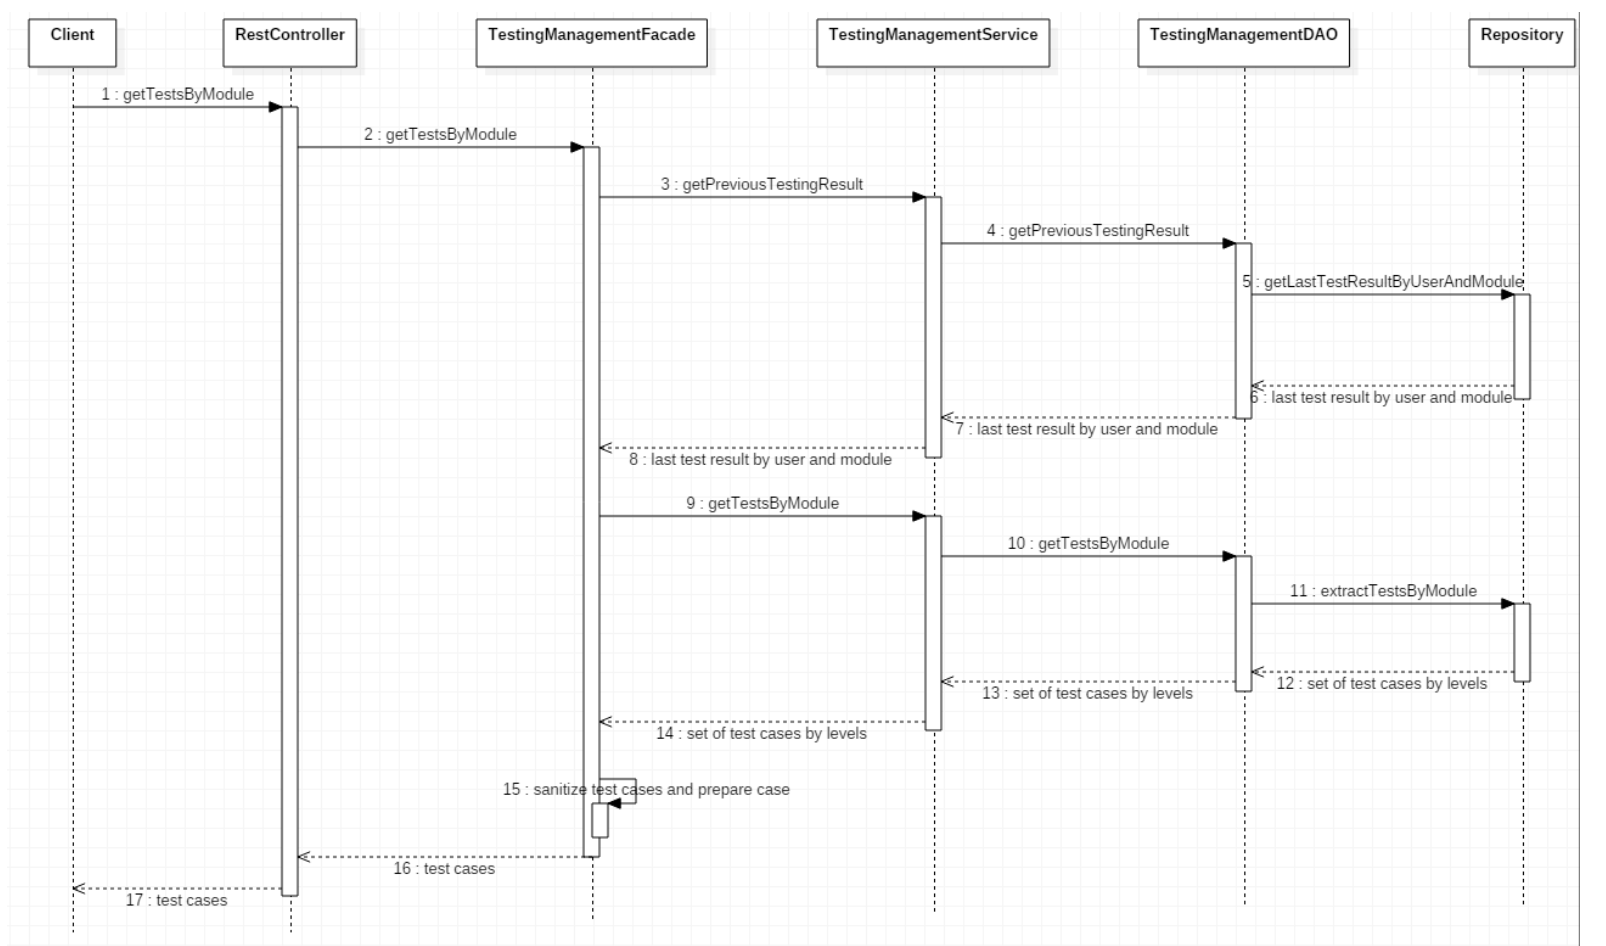
\includegraphics[width=1\textwidth]{fig6}
    \caption{Building test cases for particular module and current user}
    \label{fig:6}
\end{figure}

First things first, client request from browser is sent to the backend in order to obtain the needed test quiz. Rest controller intercepts this request and delegates the call to TestingManagementFacade.  The TestingManagementFacade obtains the previous quiz result for the module and current user. Based on this information there will be filtering that returns failed quizzes together with not started yet. Sanitized test cases are returned to the client. 

Equally important is content selection for the user. Figure~\ref{fig:7} shows the corresponding diagram.

\begin{figure}[H]
    \centering
    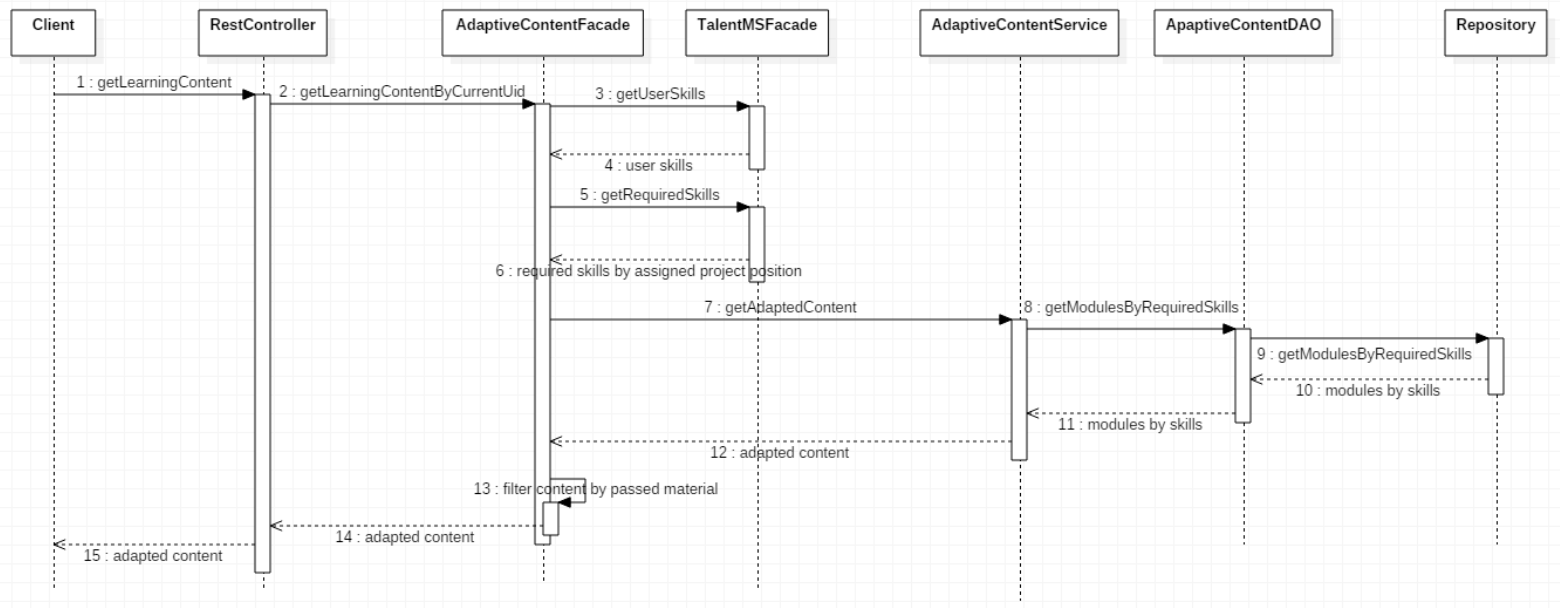
\includegraphics[width=1\textwidth]{fig7}
    \caption{Sequence diagram which reflects the choice of educational content for user}
    \label{fig:7}
\end{figure}

To obtain educational content, sequential processes are performed. 
\begin{enumerate}
    \item The client initiates a request for training material.
    \item A method that is related to the semantics of a customer request is implemented. In the middle of the method, the controller delegates the execution of the AdaptiveContentFacade facade request.
    \item AdaptiveContentFacade refers to TalentMS, which is presented in
    quality of the TalentMSFacade facade interface with a request for current knowledge of the candidate.
    \item TalentMSFacade returns the candidate's current knowledge.
    \item AdaptiveContentFacade asks TalentMS to request the required knowledge for a particular competency.
    \item TalentMSFacade returns a list of competencies.
    \item Having the current knowledge of the Candidate Candidate in need of a competency, AdaptiveContentFacade requests that the content of the competencies specified in the AdaptiveContentService be obtained.
    \item AdaptiveContentService queries knowledge content to AdaptiveContentDAO.
    \item AdaptiveContentDAO retrieves knowledge content set.
    \item AdaptiveContentDAO transmits the removed content to the AdaptiveContentService.
    \item AdaptiveContentService transmitsAdaptiveContentDAO-derived content to AdaptiveContentFacade.
    \item AdaptiveContentFacade performs so-called content filtering on the knowledge they pump and the knowledge already in the candidate. In the case of knowledge, it does not make sense to take the course again. Unnecessary content is removed and adapted content is passed to the client. 
\end{enumerate}

Corresponding content that is assigned for a particular user is shown on the on the figure~\ref{fig:8}. 

\begin{figure}[H]
    \centering
    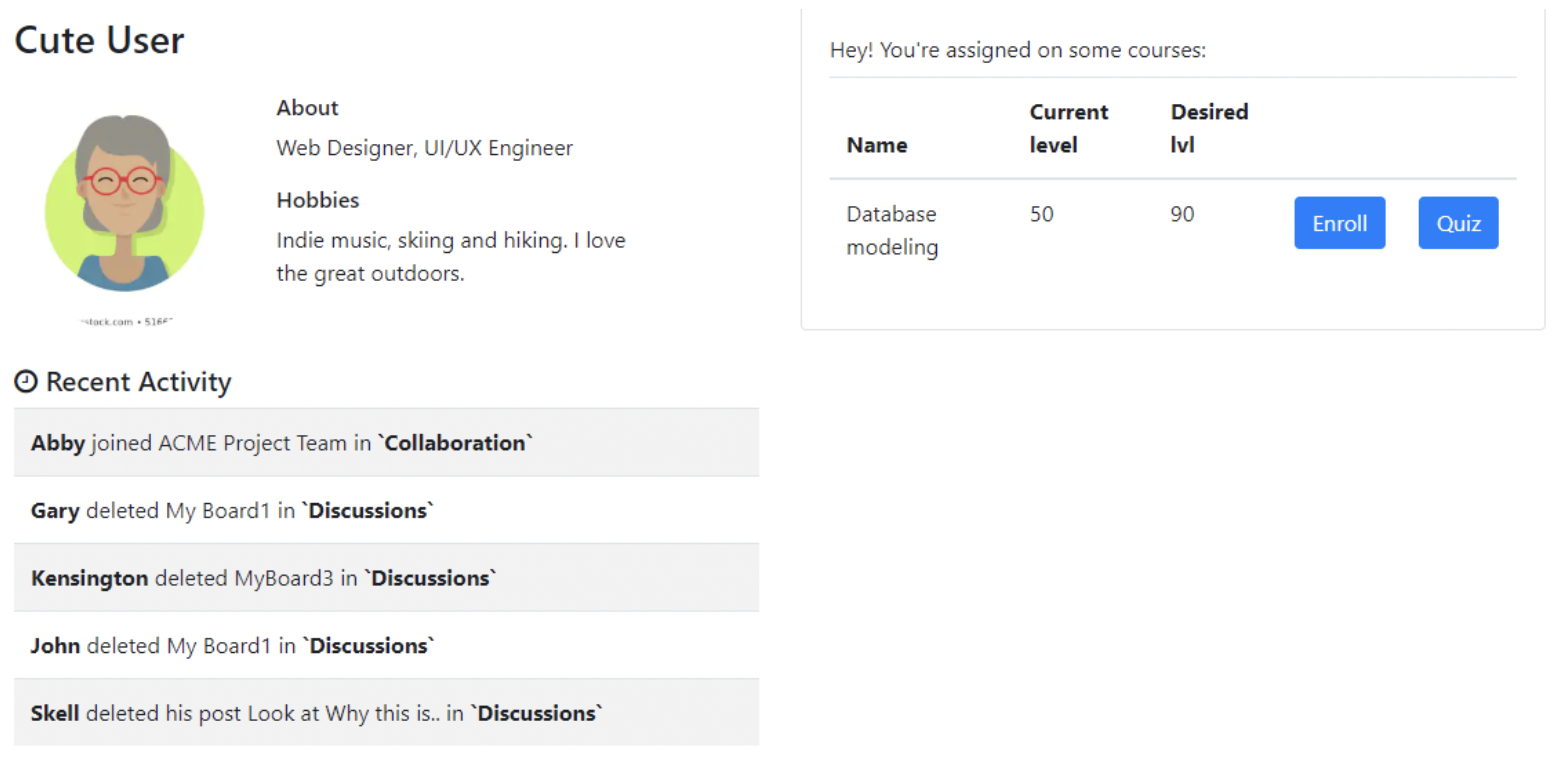
\includegraphics[width=0.7\textwidth]{fig8}
    \caption{User account with assigned adopted course}
    \label{fig:8}
\end{figure}

\section{Conclusions}
In order to achieve the goal of the thesis, the following tasks have been completed.
\begin{enumerate}
    \item The subject area was chosen for e-learning in small and medium-sized IT companies, according to which the approaches to personnel training in terms of project requirements were analyzed.
    \item The advantages and disadvantages of using corporate e-learning in the corporate sphere are identified. The purpose of such training and motivation is determined. Based on the analysis of the subject area, it is concluded that the need to develop software to implement an adaptive approach to the formation of educational content.
    \item The characteristics and classification of modern e-learning systems of the personnel are given, the general structure of such systems and their typical functionality are analyzed, which made it possible to identify ways of improvement-learning systems and corporate adaptation options.
    \item A model of competence structure display based on graph theory is proposed, an algorithm for selecting educational content for individual needs is visualized.
\end{enumerate}

Therefore, the approach for creating adoptive training content was suggested that enables resource managers to form teams automatically and according to project needs, and to provide employees with training material that corresponds their individual training level.

\printbibliography[heading=bibintoc, title={References}]

\end{document}